\documentclass[dvipsnames,xcolor, handout]{beamer}
\usepackage[spanish]{babel}
\usepackage[utf8]{inputenc}
\usepackage[all]{xy}
\usepackage{afterpage}
\usepackage{tikz}
\usepackage{cancel}
\usepackage{verbatim}
\usepackage{xfrac}
\usepackage{mathrsfs}
\usepackage{amsthm}
\usepackage{amssymb}
\usepackage{bbm}
\usepackage{enumerate}
\usepackage{booktabs}
\usepackage{relsize}
\usepackage{hyperref}
\usepackage{float}
\usetikzlibrary{decorations.pathmorphing, patterns,shapes}
\usetikzlibrary{positioning}
\usepackage{pgfplots}
\pgfplotsset{compat=1.12}
\PassOptionsToPackage{demo}{graphicx}

\usepackage{array}

\usepackage{amsmath}
\usepackage{multirow}
\usepackage{colortbl}
\usepackage{multicol}
\usepackage{adjustbox}
\usepackage{xfrac}
\usepackage{bm}

\newcommand{\tconv}{\operatorname{tconv}}
\newcommand{\type}{\operatorname{type}}
\newcommand{\Img}{\operatorname{Img}}
\newcommand{\Eig}{\operatorname{Eig}}
\newcommand{\covec}{\operatorname{coVec}}
\newcommand{\cells}{\operatorname{cells}}
\newcommand{\basic}{\operatorname{basic}}
\newcommand{\dist}{\operatorname{d}}
\newcommand{\hdist}{\operatorname{d_H}}
\newcommand{\pr}{\operatorname{pr}}
\newcommand{\random}{\operatorname{random}}

\newcommand{\hlc}[2][yellow]{ {\sethlcolor{#1} \hl{#2}} }

\newcommand*{\rom}[1]{\expandafter\romannumeral #1}
\newcommand{\Rom}[1]{\uppercase\expandafter{\romannumeral #1\relax}}

\newcommand{\Importante}[2]{{\color{#1}#2}}
\newcommand{\importante}[2]{{\color{#1}\underline{#2}}}

\renewcommand{\baselinestretch}{1}
\setlength{\parskip}{\baselineskip}


\def\Put(#1,#2)#3{\leavevmode\makebox(0,0){\put(#1,#2){#3}}}

 \usetheme{Boadilla}

%\usecolortheme{crane}
\definecolor{indigo}{rgb}{0.169,0, 0.6}
\usecolortheme[named=indigo]{structure}
\usepackage{natbib}


\theoremstyle{plain}
  \newtheorem{teorema}{Teorema}
  \newtheorem{proposicion}{Proposición}
  \newtheorem{corolario}{Corolario}
  \newtheorem{lema}[teorema]{Lema}
\theoremstyle{definition}
  \newtheorem{definicion}{Definici\'on}
  \newtheorem{ejemplo}{Ejemplo}
  
  
\makeatletter
\setbeamertemplate{footline}
{
  \leavevmode%
  \hbox{%
  \begin{beamercolorbox}[wd=.4\paperwidth,ht=2.25ex,dp=1ex,center]{author in head/foot}%
    \usebeamerfont{author in head/foot}\insertshortauthor \hspace*{1em}(\insertshortinstitute)
  \end{beamercolorbox}%
  \begin{beamercolorbox}[wd=.5\paperwidth,ht=2.25ex,dp=1ex,center]{title in head/foot}%
    \usebeamerfont{title in head/foot}\insertsection 
  \end{beamercolorbox}%
  \begin{beamercolorbox}[wd=.1\paperwidth,ht=2.25ex,dp=1ex,center]{date in head/foot}%
    \usebeamerfont{date in head/foot}
    \insertframenumber{} / \inserttotalframenumber\hspace*{2ex} 
  \end{beamercolorbox}}%
  \vskip0pt%
}
\makeatother
  
\title{Taller usos de \LaTeX \\ \small{Introducción a \LaTeX}  \vspace*{-0.2cm}}

\setbeamersize{text margin left=25pt,text margin right=25pt}

\author[Julián Chitiva Bocanegra]{Julián Enrique Chitiva Bocanegra}
\institute[Uniandes] 
{Universidad de los Andes\\ Facultad de Economía}
\titlegraphic{
\includegraphics[width=0.8cm]{img/uniandes_logo.png}
}

\date{\today}

\subject{}
\usepackage[figurename=]{caption}
\begin{document}
\begin{frame}
  \titlepage
\end{frame}

\begin{frame}{Contenido}
  \tableofcontents%[hideallsubsections]%, currentsection]
\end{frame}


\section{Introducción}
\begin{frame}{Contenido}
  \tableofcontents[currentsection]%hideallsubsections]
\end{frame}
\subsection{\textquestiondown Qué es?}
\begin{frame}{\textquestiondown Qué es?}
\begin{itemize}
    \item \textquestiondown Qué es \TeX ?\pause\\
    Es un sistema de tipografía creado por Donalth Knuth en 1978. \pause
    \item \textquestiondown Qué es \LaTeX ?\pause\\
    Es un sistema de preparación de documentos escritos en lenguaje \TeX creado por Leslie Lamport.\\
    Se usa para producir documentos de todo tipo de manera profesional. Ej: reportes, artículos, tesis, libros, presentaciones, examenes, etc.
\end{itemize}
\end{frame}

\begin{frame}{Filosofía}
    \begin{itemize}
        \item Editores de texto tradicionales se consideran ``What you see is what you get''
        
        \item \LaTeX es más ``What you see is what you mean''. Esto permite que el usuario se preocupe más por el contenido que por el formato. (No siempre)
    \end{itemize}
\end{frame}

\subsection{\textquestiondown Por qué usarlo?}
\begin{frame}{\textquestiondown Por qué usarlo?}
Ampliamente utilizado en el mundo científico. Es utilizado
por editoriales como Addison-Wesley, Elsevier, Oxfor University Press, Springer, entre otras.
\end{frame}
\begin{frame}{Ventajas y Desventajas}
    \begin{itemize}
        \item Ventajas
        \begin{itemize}
            \item Existen plantillas profesionales disponibles.
            \item Hace muy fácil la inclusión de características como referencias cruzadas, bibliografías, ambientes matemáticos, índices, etc.
            \item Facilita la correcta estructuración de un documento.
            \item Es libre y funciona en cualquier tipo de hardware.
        \end{itemize}
        \item Desventajas
        \begin{itemize}
            \item No es adecuado para documentos tales como afiches, documentos publicitarios, presentaciones publicitarias.
        \end{itemize}
    \end{itemize}
\end{frame}

\section{Instalación}
\begin{frame}{Contenido}
  \tableofcontents[currentsection]%hideallsubsections]
\end{frame}
\subsection{Aspectos básicos}
\begin{frame}{Aspectos básicos}
\begin{itemize}
    \item El documento se redacta con comandos especiales (lenguaje \LaTeX), que se compilan y producen un archivo de salida en formato pdf. \pause
    \item Cuando se hace uso de funciones especiales (insertar gráficos, utilizar lenguaje matemático, etc.) se deben importar los paquetes correspondientes. \pause
    \item Existen diversos compiladores disponibles con diferentes capacidades. \textbf{TexStudio}, \textbf{TeXShop}, TeXnicCenter, Texmaker, TeXworks y \textbf{Overleaf} ofrecen un entorno excelente para el desarrollo de documentos en \LaTeX.
\end{itemize}
\end{frame}
\subsection{Instalación}
\begin{frame}[fragile]{Instalación}
Para escribir documentos en \LaTeX es necesario instalar dos componentes. La librería de \LaTeX y un compilador del código. Esto variará según el sistema operativo.

\begin{itemize}
    \item Windows
    \begin{itemize}
        \item Librería: MikTeX \href{http://miktex.org/download}{miktex.org}
        \item Compilador: TexStudio \href{http://texstudio.sourceforge.net/}{texstudio.sourceforge.net}
    \end{itemize}
    \item Mac
    \begin{itemize}
        \item Librería: MacTeX \href{http://www.tug.org/mactex/index.html}{www.tug.org/mactex}
        \item Compilador: TexStudio \href{http://texstudio.sourceforge.net/}{texstudio.sourceforge.net}
    \end{itemize}
    \item Linux
    \begin{itemize}
        \item Librería: TexLive \begin{verbatim}sudo apt-get install texlive-full\end{verbatim}
        \item Compilador: TexStudio \href{http://texstudio.sourceforge.net/}{texstudio.sourceforge.net}
    \end{itemize}
\end{itemize}
\end{frame}

\begin{frame}{Instalación}
\begin{itemize}
    \item Hay algunos compiladores de \LaTeX\ que no requieren instalación.
    \item El más conocido es \href{http://overleaf.com}{overleaf}
\end{itemize}
\end{frame}

\subsection{Estructura básica de un compilador}

\begin{frame}{Estructura básica de un compilador: local}
    \begin{figure}
        \centering
        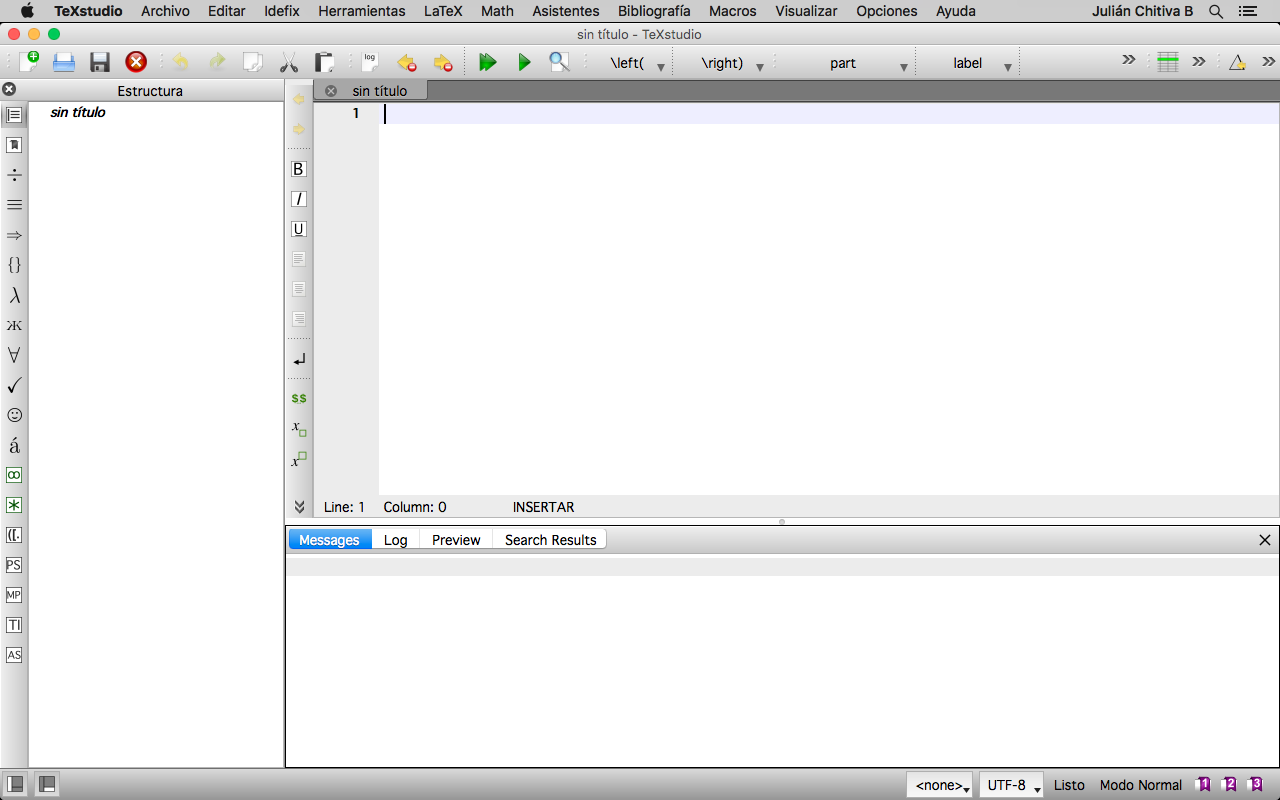
\includegraphics[width=\linewidth]{img/clase1_texstudio.png}
        \caption{Ambiente de TexStudio}
        \label{fig:texstudio}
    \end{figure}
\end{frame}

\begin{frame}{Estructura básica de un compilador: on-line}
    \begin{figure}
        \centering
        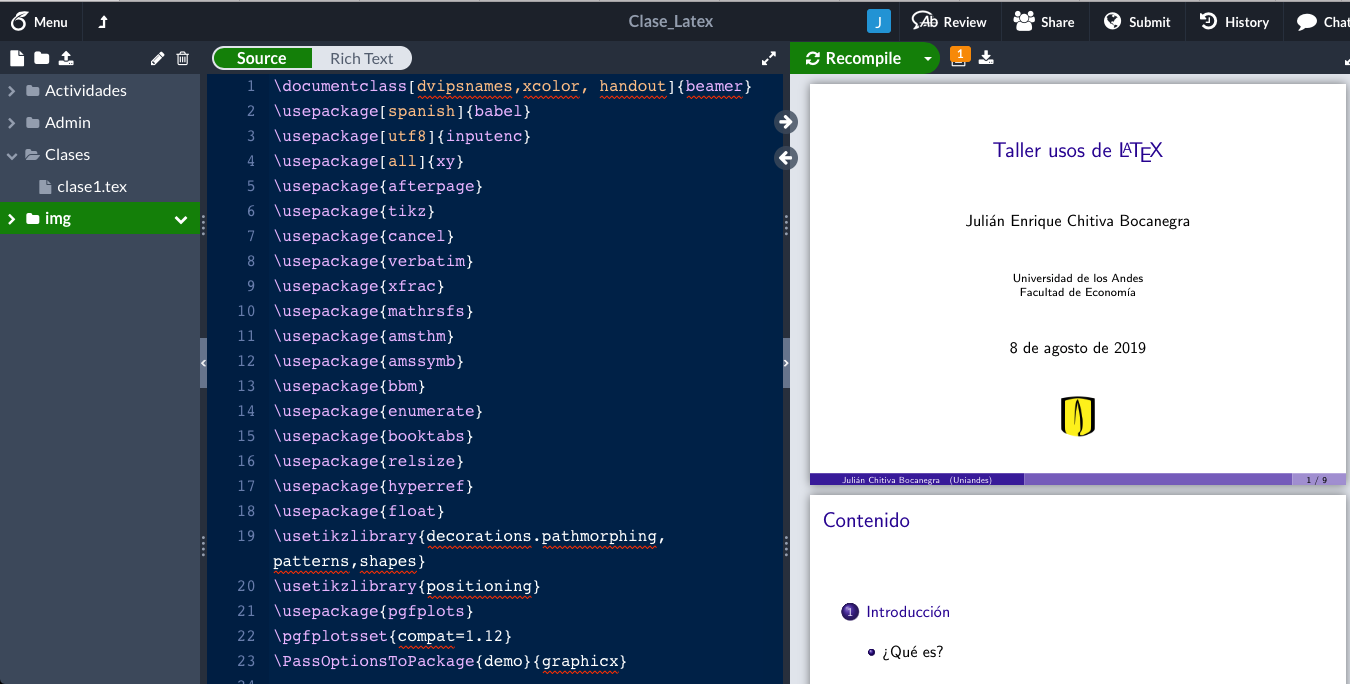
\includegraphics[width=\linewidth]{img/clase1_overleaf.png}
        \caption{Ambiente de overleaf}
        \label{fig:texstudio}
    \end{figure}
\end{frame}
\begin{frame}
    Un compilador cuenta con diversas características para facilitar la escritura de un documento. Las más importantes son:
    \begin{itemize}
        \item Campo para escritura del documento 
        \item Ventana de navegación del documento (Overleaf no tiene esto)
        \item Cuadro de mensajes
        \item Múltiples barras de herramientas (Overleaf no tiene esto)
        \item Campo para la visualización del documento.
    \end{itemize}
\end{frame}

\section{Documentos}
\begin{frame}{Contenido}
  \tableofcontents[currentsection]%hideallsubsections]
\end{frame}
\subsection{Estructura básica de un documento}
\begin{frame}[fragile]{1. Clase}
\begin{verbatim}
    \documentclass[opciones]{clase}
\end{verbatim}
\vspace*{-0.5cm}
\begin{itemize}
    \item Siempre va en la primer linea. Define el tipo de documento que se desea construir. 
    \item Dependiendo del tipo de documento se cargarán ciertas funciones.
    \item Clases más comunes:
    \begin{itemize}
        \item Article: cualquier documento corto (es la más usada).
        \item Book: documentos de gran extensión.
        \item Beamer: presentacion con diapositivas.
    \end{itemize}
    \item Opciones mas comunes:
    \begin{itemize}
        \item Tamaño de letra: 10pt, 11pt, 12pt
        \item Tamaño de hoja: a4paper, letterpaper
        \item Multiples columnas: onecolumn, twocolumn
    \end{itemize}
    \item Ejemplo:
\end{itemize}
\vspace*{-0.5cm}
\begin{small}
\begin{verbatim}
        \documentclass[12pt, letterpaper, twocolumn]{article}
    \end{verbatim}
\end{small}

    
\end{frame}

\begin{frame}[fragile]{2. Preámbulo}
\begin{verbatim}
    \usepackage[opciones]{paquete}
\end{verbatim}
\vspace*{-0.5cm}
\begin{itemize}
    \item Carga los paquetes que se necesarios para la compilación del documento.
    \item Se pueden definir comandos globales.
    \item Paquetes más comunes
    \begin{itemize}
        \item Codificación del texto
        \begin{verbatim}\usepackage[utf8]{inputenc}\end{verbatim}
        \item Define los títulos predefinidos en español
        \begin{verbatim}\usepackage[spanish]{babel}\end{verbatim}
        \item Carga paquetes de escritura de ecuaciones
        \begin{verbatim}\usepackage{amsmath, amsfonts, amssymb}\end{verbatim}
        \item Ajusta las márgenes.
        \begin{verbatim}\usepackage[left=2cm, right=2cm,
        top=2cm, bottom=2cm]{geometry}\end{verbatim}
    \end{itemize}
\end{itemize}
    
\end{frame}

\begin{frame}[fragile]{3. Cuerpo}
\begin{verbatim}
    \begin{document}
     Contenido ...
    \end{document}
\end{verbatim}
\vspace*{-0.5cm}
\begin{itemize}
    \item Delimita el contenido del documento
    \item Aqui se redacta el texto, se incluyen gráficos y se desarolla el contenido.
\end{itemize}
    
\end{frame}

{ % all template changes are local to this group.
    \setbeamertemplate{navigation symbols}{}
    \setbeamercolor{background canvas}{bg=indigo}
    \begin{frame}[plain, noframenumbering]
    \vfill
    \begin{center}
    \begin{Huge}
        %\textcolor{white}{Gracias!}
    \end{Huge}
    \end{center}
    \vfill
     \end{frame}
}

\end{document}